% Frozen evidence: manuscript/evidence/2026-10-24_spatial_revision/spacing_conformers.json
\begin{frame}{One intervening repeat still permits motif contact}
\centering
% Show the two one-spacer panels at readable size; the full four-panel figure
% and exact coordinate/source data remain in the checked manuscript snapshot.
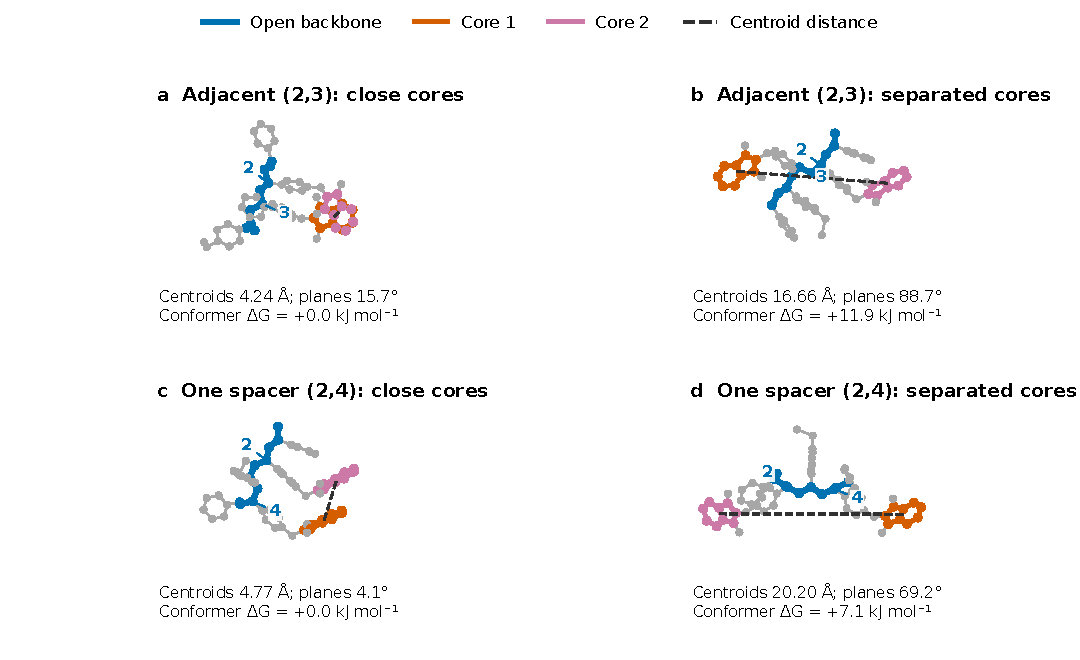
\includegraphics[width=.96\linewidth,height=.61\textheight,keepaspectratio,trim=0 0 0 158pt,clip]{../results/figures/manuscript/2026-10-24_spatial_revision/spacing_conformers.pdf}
\par\smallskip\small
Blue: open backbone. Orange/magenta: grafted core rings at sites 2 and 4.
\par\smallskip\small
Within this two-conformer phthalimide set, the close-contact state has lower $G$ by 7.1 kJ/mol.
\par\smallskip\footnotesize
The difference includes the entire chain and solvent response. Broader conformer convergence, isolated motif binding and electronic coupling remain separate requirements.
\end{frame}
